% Analyzujte nové síťové architektury jako Recursive InterNetwork Architecture (RINA) a Named Data Networking.
% Popište současný stav nasazení těchto architektur v reálném provozu i v prostředí OMNeT++. Popište jejich výhody/nevýhody.
% Implementujte modul Relaying and Multiplexing Task z RINA v prostředí OMNeT++ podle požadavků vedoucího.
% Vytvořte sadu příkladů pro demonstraci Vaší implementace. Zhodnoťte Vaše výsledky.


\chapter{Introduction}\label{intro}

    Today's field of computer networking and its research is heavily centered around the underlying architecture of the Internet and its protocol suite, which is known as TCP/IP for its two most prominent protocols Transmission Control Protocol (TCP) and Internet Protocol (IP). While such concepts are in use for several decades and seem to work as intended, there has been a growing trend in the research community of introducing new alternative network architectures. This thesis aims to illustrate aims of such architectures and contribute to implementation of one of them.

    Network simulation is an ideal approach for examining new network architectures since it provides a quick and efficient way of setting up test scenarios and observing all aspects of their behavior. The discrete event network simulation framework OMNeT++ has been chosen as the target implementation platform.

    \section{Goals}

        The theoretical part of this thesis aims to describe some alternatives to the currently prevalent network architectures. Since the Internet is by far the largest and most important example of an internetwork, its underlying architecture shall be used as a base for comparison. This is only fitting since nearly all of the recent network architecture research is directed towards improving the Internet. Description of each architecture includes information about prototyping efforts, both in real-life platforms and in the field of network simulation.

        The technical report describes design and implementation of a component of one of the presented architectures, Recursive InterNetwork Architecture (RINA), for the OMNeT++ framework.

    \section{Thesis Structure}

        Chapter \ref{problems} describes the shortcomings and weak parts of current Internet technology which create the need for alternative architecture research. This overview serves in later chapters as a reference point for evaluating contributions of alternative architectures.

        Chapter \ref{archs} presents an outline of current projects in field of network architecture and describes a representative set of architectures.

        Chapter \ref{comparison} sums up and evaluates contributions brought by the previously described architectures.

        Chapter \ref{forwarding} takes a closer look at parts of RINA that are related to the implementation.

        Chapter \ref{implementation} describes implementation of RINA's Relaying and Multiplexing Task (RMT) for OMNeT++.

        Chapter \ref{testing} presents evaluation of the implementation in form of sample test scenarios and their outputs.


\chapter{Problems of The Current Internet}\label{problems}

    The Internet could be considered one of the most important technological achievements of the 20th century. It has brought a previously unimaginable degree of interconnection and information access to the whole world and its importance keeps growing even decades after its inception. Nevertheless, the very basic core of its technology was constructed over three decades ago in the era of first small experimental networks such as ARPANET and CYCLADES \cite{Kurose}, when the the demands on internetworking capabilities were nowhere compared to now.

    During the Internet's growth, whenever there has been a problem that required a solution, it's been usually dealt with in a non-intrusive evolutionary fashion by applying a new principle on top of the underlying technology. In another words, problems have been mostly solved by adding a new protocol to the TCP/IP protocol stack.

    The Internet's evolution can be presented on EvoArch \cite{EvoArch}, an abstract model for studying protocol stacks and their evolution. The model suggests that the Internet protocol stack resembles an hourglass (see Figure \ref{fig:inet_hourglass}). While the top and down layers are often expanded with new protocols, the usage of the Internet Layer's IP protocol remains constant because it acts as a common technology for all different networks interconnected by the Internet.

    \begin{figure}[H]
        \begin{center}
            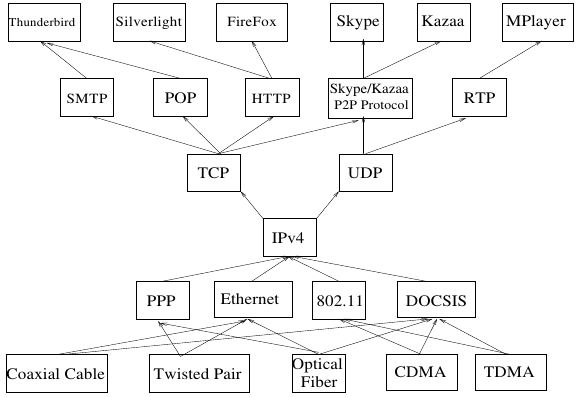
\includegraphics[width=0.5\textwidth]{fig/problems_hourglass.png}
          \caption{Internet's ``hourglass architecture''.}
          \label{fig:inet_hourglass}
        \end{center}
    \end{figure}


    The evolutionary approach to improving the Internet's base technology is convenient since each paradigm shift in foundations of the Internet (i.e. replacing the hourglass's ``thin waist'') can require a long and expensive transfer of existing network configurations to the new technology. The most notable example is is the internet layer protocol IPv6 which requires explicit firmware support from active network components. The problem of IPv4 space exhaustion has been known of since the first half of 1990s \ref{rfc1631}, the first formal IPv6 specification arose in 1998 \ref{rfc2460} and the first IPv6 routers emerged in 2004 -- and yet, as of April 2015, four years after the top-level IPv4 pool exhaustion \cite{ipv4_exhaustion}, IPv6 still represents only a miniscule fraction of the total traffic on the Internet. For example, Google IPv6 adoption statistics indicate around 6\% coverage amongst the users of its services \cite{ipv6stats}.

    As such, some of the Internet's widely recognized problems are inherent because of the base design and it's usually difficult, if not impossible, to solve them in a non-intrusive and backward-compatible way. The following sections illustrate such problems.

    \section{Incomplete naming scheme}\label{problems:naming}

        In 1982, Jerome Saltzer in his work ``On the Naming and Binding of Network Destinations'' \cite{rfc1498} described the entities and the relationships that make a complete naming and addressing schema in networks. According to Saltzer, there are four elements that need to be identified: applications, nodes, points of attachment to the network (PoAs) and paths. The relationships between them are illustrated in Figure \ref{fig:saltzer}. At the time, network architectures such as CYCLADES \cite{Cyclades}, XNS, DECNET and OSI conformed to this scheme \cite{internet_demo}.

        \begin{figure}[H]
            \begin{center}
                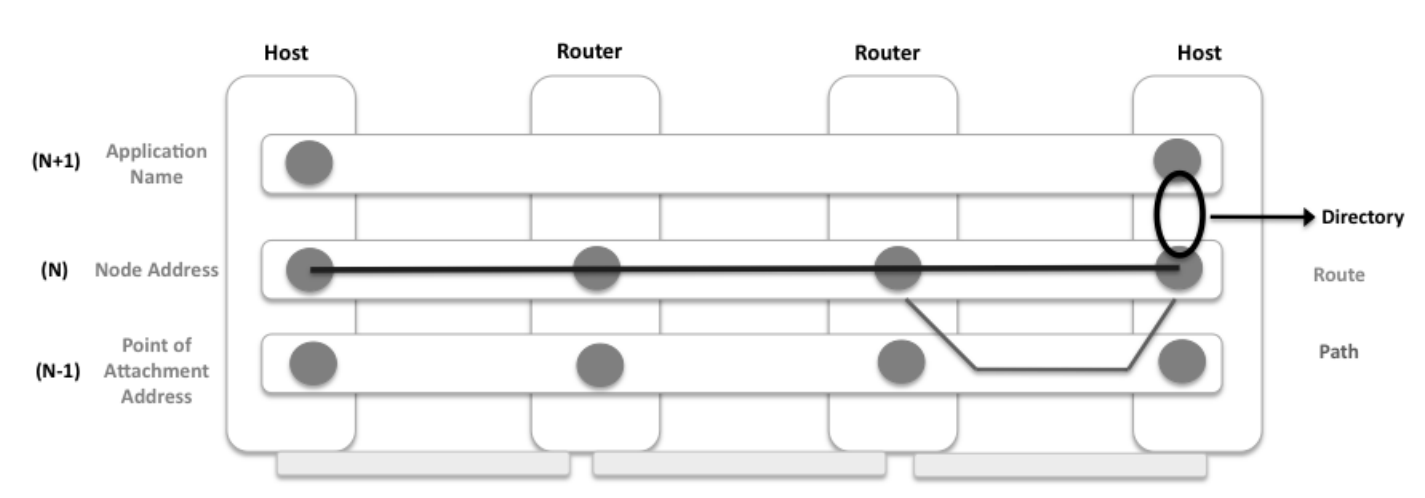
\includegraphics[width=0.8\textwidth]{fig/problems_saltzer.png}
              \caption{Jerome Saltzer's view of computer networking.}
              \label{fig:saltzer}
            \end{center}
        \end{figure}

        TCP/IP doesn't follow this proposal: the layer for node naming is completely missing. While TCP/IP does work with two distinct layers with their own address scopes -- the Link Layer with physical addresses and the Internet layer with IP addresses -- both effectively identify the same: a host interface, i.e. a PoA address. This effectively means that the IP addressing is semantically overloaded to represent both identity and location. The need for an explicit identifier$\rightarrow$locator mapping was eventually recognized even in the era of ARPANET and this was solved by creating a globally available file \texttt{HOSTS.TXT} containing mappings of alphabetic host names to IP addresses. Later on, this method was obsoleted by the Domain Name System (DNS) \cite{rfc1034}. However, both approaches move the matter of node naming into the Application Layer, forcing applications to work with location-dependent interface PoA addresses.

        The fact that the Internet forwarding is location-based instead of identity-based has a great impact on difficulty of multihoming\footnote{Multihoming refers to a computer or device connected to more than one computer network. Such computer of device generally needs a separate interface for each network.} (section \ref{problems:multihoming}) and mobility (section \ref{problems:mobility}).

    \section{Lack of Multihoming}\label{problems:multihoming}

        Since IP addresses serve as point-of-attachment addresses (i.e. an IP address identifies a system interface) and routing is done exclusively on IP's layer, there isn't any inherent mechanism for distinguishing whether multiple IP addresses identify a common node. Thus, in effect, multihoming on IP alone isn't feasible.

        The insufficient base for multihoming support is one of the oldest recognized problems of the Internet: it has become apparent back in 1972, when Tinker Air Force Base joined ARPANET and voiced a request for redundant connections to a single node to ensure reliability \cite{Patterns}. In spite of this, the switch to a new protocol suite that happened 11 years later (on 1.1.1983, the ``flag day'') didn't bring any solution to this problem.

        Since then, some attemps were made to implement multihoming on top of the current architecture.

        \begin{itemize}
            \item \textbf{SCTP.}
            Message-oriented transport protocol Stream Control Transmission Protocol (SCTP) \cite{rfc4960} provides a partial support. Two SCTP hosts are able to provide each other with lists of alternate IP addresses that can be used as fallback points of attachment of the same application in case of failure of the primary address. During such session, each SCTP host needs to continually check other host's endpoints by heartbeat packets to make sure they are accessible via other sessions.
            However, thus far, multiple reasons have been preventing SCTP from becoming a widely known and used solution; the biggest disadvantage lies in the fact that due to TCP/IP not having a distinct session layer on top of its transport layer (such as in ISO/OSI stack), the transport protocol has to be explicitly specified by the application using the BSD sockets Advanced Programming Interface (API). Therefore, SCTP adoption would require a rewrite of network-aware applications themselves. Other SCTP adoption issues include unsatisfactory operating system support (Microsoft Windows systems require a third-party kernel driver) and weak awareness of its existence outside the networking community.

            \item \textbf{BGP Multihoming.} Another implementation of multihoming capabilities can be seen in Border Gateway Protocol (BGP) \cite{rfc4271}, which provides means for load-balancing and fallback over multiple links on T1 networks. To make use of such multihoming over the Internet, a public IP address range and an Autonomous System number are required. BGP Multihoming is one of the most significant causes contributing to the growth of Internet routing table.

            \item \textbf{Multipath TCP.} The most recent TCP/IP multihoming initiative is the TCP extension Multipath TCP (MPTCP) which is currently in its experimental phase, although a large scale commercial deployment has been already made by Apple for its Siri network application in mobile operating system iOS 7 \cite{Apple_MP}.
        \end{itemize}

    \section{Lack of Mobility}\label{problems:mobility}

        Since a host location is determined by its IP address and IP addressing is location-dependent, mobility is essentialy non-existent.

        There have been three distinct approaches to solving the mobility problem \cite{MobilityFirst}.

        \begin{itemize}
            \item \textbf{Mobility by indirection.} A fixed host is dedicated for keeping track of mobile devices and forwarding traffic to them. This leads to path inflation.
            This approach is used by technologies such as Mobile IP \cite{rfc5944} or Locator/Identifier Separation Protocol (LISP) \cite{rfc6830}.
            \item \textbf{Global name resolution.} The endpoint identifier is resolved to its network location by looking up a logically centralized service.
            This approach is used by technologies such as eXpressive Internet Architecture (XIA) \cite{xia} (described in section \ref{archs:xia}) or MobilityFirst \cite{MobilityFirst} (described in section \ref{archs:mf}).
            \item \textbf{Name-based routing.} The network locator is completely disregarded and routing is done directly on names.
            This approach is used by technologies such as Named Data Networking (NDN) \cite{ndn} (described in section \ref{archs:ndn}) or TRIAD.
        \end{itemize}

        The second and third approaches require a clean-slate architectural design.

    \section{Lack of security mechanisms}\label{problems:security}

        The specifications of the fundamental protocols of TCP/IP stack -- IP, TCP and DHCP -- were originally finished at the beginning of 1980s. The Internet has since then turned into a massive world-wide internetwork connecting people of different types and agendas. Naturally, once the Internet began to be used for transferring sensitive data (especially by companies), cyber crime started to emerge as well and some attention was turned to security aspects of Internet protocol (or lack thereof).

        As the IP protocol lacks any inherent verification mechanism, the Internet Layer is easily subjected to hijacking and spoofing. This provides opportunity for many types of exploits, most notably the  Man-in-the-middle attack or IP address spoofing \cite{rfc1948}.

        Since security isn't enforced by the architecture in any way, it's still common even for the Application Layer with its plethora of protocols to be subjected to security problems. Protocols like TCP are still widely in use and remain vulnerable to attacks such as TCP sequence prediction attack \cite{rfc1948}.


    \section{Router Table Size Growth}

        Default-free zone (DFZ) is the collection of all Internet autonomous systems (ASs) that do not require a default route to forward a packet to any destination. Since they comprise the root of the Internet's routing infrastructure, their database must be complete.

        With the increasing number of hosts connected to the Internet, the DFZ routing table sizes grow as well (see Figure \ref{fig:bgp-growth}).

        \begin{figure}[H]
            \begin{center}
                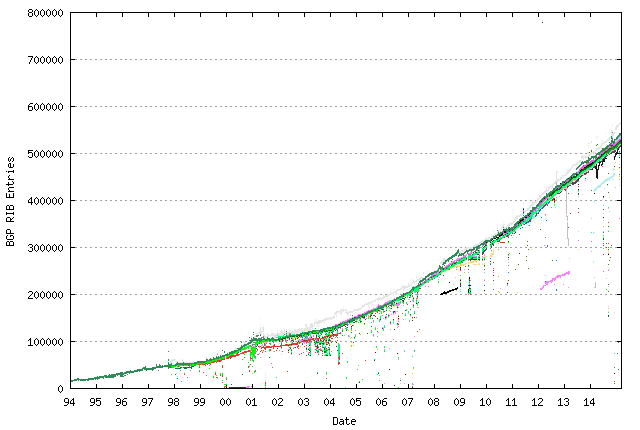
\includegraphics[width=0.6\textwidth]{fig/problems_bgp-growth.png}
              \caption{Global Internet routing table size growth \cite{bgpgrow}}
              \label{fig:bgp-growth}
            \end{center}
        \end{figure}

        While the exponential growth observed during the 1990s was later mitigated by mass deployment of Classless Inter-Domain Routing (CIDR) and BGP route aggregation, the number of items is still increasing superlinearly and the high-end router hardware needs to keep up, especially with increasing use of BGP-based multihoming and IPv6. This can sometimes lead to scalability problems, as in August of 2014 where reaching the 512k entry limit of multiple routers caused globally observable outages \cite{512k_day}.

        As of year 2015, the Internet routing table consists of over 560k entries \cite{bgpgrow}. There are concerns about whether the technology of high-end routers will keep scaling along with Moore's law to keep route management efficient \cite{rfc4984}.


\chapter{Alternative Network Architectures}\label{archs}

    This chapter gives an overview of paths that were pursued in the field of network architecture research and descriptions of several architectures.

    Considering the limited scope of this thesis, only a representative subset of new network architectures will be described and evaluated more thoroughly. The subset consists of projects funded by the Future Internet Architecture -- Next Phase program \cite{fia} (Named Data Networking [Section \ref{archs:ndn}], MobilityFirst [Section \ref{archs:mf}] and eXpressive Internet Architecture [Section \ref{archs:xia}]) and the Recursive InterNetwork Architecture (\ref{archs:rina}).

    Special attention will be given to Recursive InterNetwork Architecture as it's relevant to the implementation goal of this thesis.

    \section{Design Approaches}

        The networking research community has exhibited many attempts of moving the field forward. The undertaken research directions are often classified into one of two groups:

        \begin{itemize}
            \item \textbf{Evolutionary design.} Backward-compatible solutions that are incrementally deployable on top of the current Internet (e.g. LISP, DiffServ or IntServ).
            \item \textbf{Clean slate design.} Completely new standalone architectures that aren't constrained by Internet technology's limitations (e.g. NDN, RINA).
        \end{itemize}

        Considering the scope of this thesis, the focus will be given exclusively to ``clean-slate design'' architectures.

    \section{Named Data Networking}\label{archs:ndn}

        Named Data Networking is one instance of a more general research direction called Information-centric networking (ICN) \cite{icn}. ICN explores the possibilities of moving the Internet infrastructure away from its host-centric communication paradigm towards the idea of named content.

        \subsection{Premise}

            During its early ears, ARPANET was heavily influenced by telecommunication technology as the Public switched telephone network (PSTN) was the only example a large-scale network. Due to this, technology of the Internet has been built on the paradigm of host-to-host communication driven by hosts' addresses. However, while this base paradigm has remained constant over the decades, the way we use the Internet has considerably changed: the Internet is used primarily as a content distribution network. Since the mechanism of communication over the Internet is based on creating and maintaining end-to-end connections, this creates an enormous amount of data redundancy.

            Named Data Networking proposes a solution more fitting for today's needs: instead of working with the source/destination addresses, the ``thin waist'' of the Internet should be based on working with names of data chunks (as illustrated by Figure \ref{fig:ndn_waist}).

            \begin{figure}[H]
                \begin{center}
                    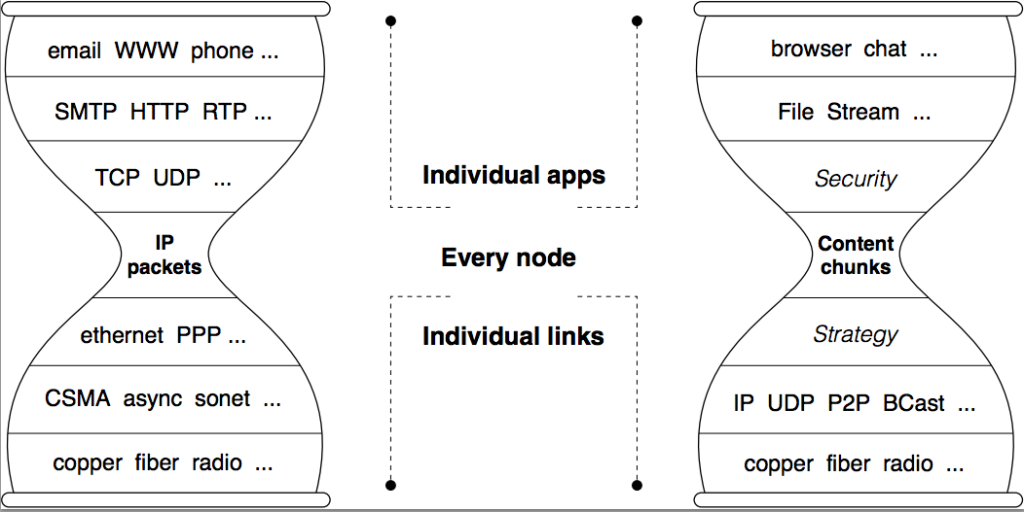
\includegraphics[width=0.7\textwidth]{fig/archs_ndn-hourglass.png}
                  \caption{``Thin waists'' of the current Internet and NDN.}
                  \label{fig:ndn_waist}
                \end{center}
            \end{figure}

        \subsection{Concepts}

            \subsubsection{The Building Blocks}

                The NDN architecture specifies:
                    \begin{itemize}
                        \item two types of packets: an interest packet (containing the name of desired data) and a data packet (containing the requested data),
                        \item two types of hosts: a consumer (data requester) and a producer (data provider), and
                        \item a router maintaining three fundamental data structures:
                        \begin{itemize}
                            \item Forwarding Information Base (FIB) (forwarding table)
                            \item Pending Interest Table (PIT) (maintaining currently active requests)
                            \item Content Store (data cache)
                        \end{itemize}
                        \begin{figure}[H]
                            \begin{center}
                                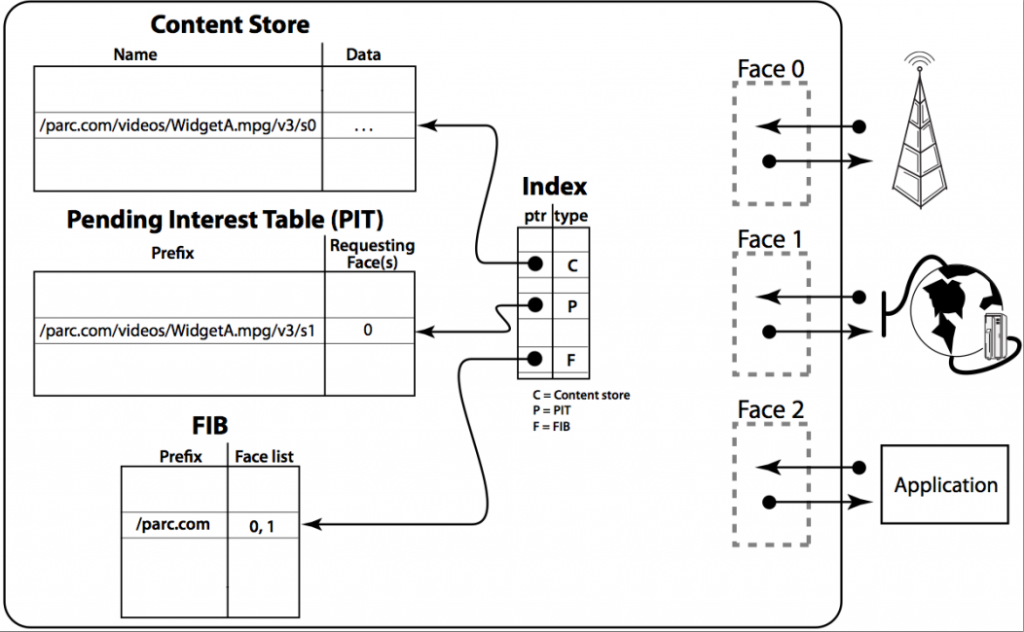
\includegraphics[width=0.6\textwidth]{fig/archs_ndn-router.png}
                              \caption{NDN router.}
                              \label{fig:ndn-router}
                            \end{center}
                        \end{figure}

                    \end{itemize}

            \subsubsection{The Communication Model}

                Communication in NDN is driven by the data receiver, i.e. the consumer. The steps are:

                \begin{enumerate}
                    \item The consumer sends out an interest packet containing the name of the desired data.
                    \item When a router receives the interest packet, it first consults its Content Store for requested data.
                        \begin{itemize}
                            \item If the data requested by the interest packet are present, they are returned in the direction of the requesting interface.
                            \item Otherwise, it'll look up the PIT.
                            \begin{itemize}
                                \item If there's an entry present for the named data request, the entry is updated by adding the originating interface into the list of requesting interfaces, thus aggregating the new request together with an existing one.
                                \item Otherwise, a new entry is inserted, a FIB lookup is made and the interest packet is forwarded to interface(s) returned by the FIB.
                            \end{itemize}
                        \end{itemize}
                    \item A data packet is returned to the router by either the producer or another router with cached data. The router finds a matching PIT entry and forwards the data to all interfaces listed in the PIT entry. The PIT entry is then removed and data are cached into the Content Store.
                \end{enumerate}

            \subsubsection{Naming}

                NDN assumes data chunk names to be hierarchically structured. Consumers must be able to deterministically construct the name for a desired piece of data without having previously seen the name or data. This can be achieved either by a deterministic algorithm allowing both consumer and producer to construct the same name based on data available to both.

                The management of such namespace isn't defined by the architecture itself and should be a subject of further research.

        \subsection{Current State of Implementation}

            NDN's implementation efforts are open-source and available as a package called \texttt{NDN Platform} \cite{ndn_platform}. The package contains a C++ library (\texttt{ndn-cxx}), the NDN Forwarding Daemon (\texttt{NFD}), client libraries for C++, Python, Java and JavaScript, NLSR routing protocol, NDN repository and additional networking tools (a ping-like application, a traffic generator and a traffic capture tool).

            \texttt{ndnSIM} \cite{ndn_sim}, based on \texttt{ns-3} \cite{ns3}, is a network simulator using \texttt{ndn-cxx} and \texttt{NFD} as the architecture backend. ndnSIM extends ns-3 with a new network-layer protocol model which can be used atop of any available link-layer protocol, thus providing a flexible solution for simulating various development scenarios.


    \section{MobilityFirst}\label{archs:mf}

        \subsection{Premise}

            The current Internet is designed for interconnecting fixed endpoints and fails to address dramatically increasing demands of mobile devices and services. MobilityFirst, as its name would suggest, aims to provide means for better mobility, while also introducing intristic security properties and faciliating services.

        \subsection{Concepts}

            MobilityFirst is based on three basic principles: separation of locator and identifier (i.e. node name and PoA address), intristic security and global name resolution.

            \subsubsection{Loc/ID Separation}

                MobilityFirst's ``thin waist'' consists of location-independent names and a global name service for mapping them to addresses. A name is a globally unique identifier (GUID) that can be used to identify a variety of principals such as an interface, a node, a service, an end-user or content. An example of a principal is a network address (NA), a network identifier resembling today's autonomous sytems.

            \subsubsection{Intristic Security}

                GUIDs are self-certifying, so any principal can authenticate another principal without relying on an external authority. This is achieved through bilateral challenge-response mechanism.

                e.g. Principal X wants to verify authenticity of principal Y before establishing a connection to him.
                \begin{enumerate}
                    \item X sends a random nonce n to Y
                    \item Y responds with {pubkey, privkey(nonce)}
                    \item If hash(pubkey) == Y and pubkey(privkey(nonce)) == n, Y is authenticated
                \end{enumerate}

                % \begin{algorithm}[H]
                % \SetAlgoLined
                % \KwData{this text}
                % \KwResult{verified authenticity of Y}
                % initialization\;
                % \While{not at end of this document}{
                % read current\;
                % \eIf{understand}{
                % Y is authenticated
                % }{
                % go back to the beginning of current section\;
                % }
                % }
                % \caption{How to write algorithms}
                % \end{algorithm}

            \subsubsection{Name resolution}

                MobilityFirst defines a naming service for dynamic mapping of GUIDs to network addresses with real-time response latencies. Unlike today's Domain Name System with its reliance on a single root authority (ICANN), the naming service is decentralized.

                In addition to this, a principal can also be assigned an optional human-readable name which is bound to its public key via a name certificate. In this case, the certificate has to be obtained from a trusted certification authority.

                The system encompassing both the name resolution service and the name certification service is called the Global Name System (GNS).

            \subsubsection{The Communication Model}

                \begin{enumerate}
                    \item To contact a GUID, the sending endpoint queries the GNS to obtain an NA corresponding to a GUID (much like it queries DNS to obtain an IP address for a domain name).
                    \item The sending endpoint then begins sending data, using the tuple [GUID, NA] (which is a routable destination identifier) in packet headers.
                \end{enumerate}

                Senders can also send a packet addressed just to a GUID, thereby implicitly delegating to the first-hop router the task of querying the name service for an NA.

        \subsection{Current State of Implementation}

            \begin{itemize}
                \item msocket, an endpoint socket library extending the BSD sockets API
                \item Auspice, a GNS implementation
                \item two prototypes of the forwarding plane: one based on the Click modular router \cite{click}, other based on OpenFlow \cite{openflow}
            \end{itemize}

    \section{eXpressive Internet Architecture}\label{archs:xia}

        \subsection{Premise}

            As presented in the previous sections, some of the future architecture research is centered around the idea of replacing Internet's ``thin waist'' of end-to-end communication with a different principal or a set of principals (e.g. NDN and its named content). eXpressive Internet Architecture (XNA) takes this approach one step further and builds on one basic premise: the ``thin waist'' should provide support for multiple principals and the ability to evolve by accomodating new principals over time.

        \subsection{Concepts}

            XIA is built around three basic principles: evolvable thin waist (achieved by configurable principal types), intristic security and flexible addressing mechanism (achieved by DAG Addressing).

            \subsubsection{Principal Types}

                An XIA principal is specified by the semantics of communicaton between principals, the processing that is required to forward traffic with addresses of its type and the intristic security properties. The initial XIA architecture defines four basic XIA principal types:

                \begin{itemize}
                    \item Host XID (HID): HIDs support unicast host-based communication similar to IP where the host identifier is a hash of the host’s public key. HIDs define who you communicate with.
                    \item Service XID (SID): SIDs support communication with (typically replicated) services and realize anycast forwarding scheme. SIDs define what entities do.
                    \item Content XID (CID): CIDs allow hosts to retrieve content from ``anywhere'' in the network, e.g., content owners, CDNs, caches, etc. CIDs are defined as the hash of the content, so the client can verify the correctness of the received content. CIDs define what it is.
                    \item Network XID (NID): NIDs specify a network, i.e., an autonomous domain, and they are primarily used for scoping. They allow an entity to verify that it is communicating with the intended network.
                \end{itemize}

                Apart from above, other basic types have been introduced and experimented with, e.g. 4IDs replicating IPv4 addresses.

            \subsubsection{Intristic Security}

                Security properties are included in principal type definitions and entity validation is achieved through use of self-certifying identifiers.

            \subsubsection{DAG Addressing}

                Addressing in XIA is realized by using Directed Acyclic Graphs (DAGs). In their simplest form, address DAGs may be used only for specifying packet's destination ID as in traditional network architectures (\ref{fig:xia_dag}a). However, in addition to that, they can also contain scoping information (e.g. target network + a service located in the network [\ref{fig:xia_dag}b]) or fallback alternatives (e.g. Network XID to be used by forwarding when given SID isn't recognized [\ref{fig:xia_dag}c]).

                \begin{figure}[H]
                    \begin{center}
                        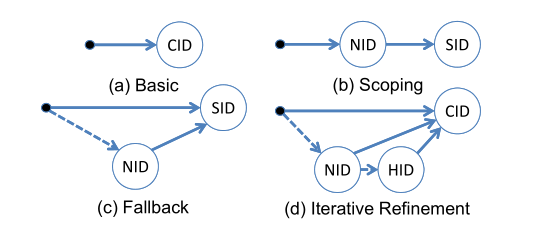
\includegraphics[width=0.6\textwidth]{fig/archs_xia-dag.png}
                        \caption{DAG-based addressing in XIA}
                        \label{fig:xia_dag}
                    \end{center}
                \end{figure}

        \subsection{Current State of Implementation}

            \begin{itemize}
                \item a Click-based prototype, including the XIA protocol stack, routing, nameserver and API
                \item a native Linux network stack implementation with attempts to port different architectures to XIA
            \end{itemize}

    \section{Recursive InterNetwork Architecture}\label{archs:rina}

        Recursive InterNetwork Architecture (RINA) is an architecture based on a set principles described by John Day in his book Patterns in Network Architecture \cite{Patterns}.

        \subsection{Premise}

            RINA introduces a novel approach to the problem of computer networking, eliminating all problems described in chapter \ref{problems} in the process:

            \begin{quotation}
                \centering
                Computer networking is a recursively scalable set of distributed applications specialized to do inter-process communication.
            \end{quotation}

        \subsection{Concepts}

            RINA specifications define a rich set of new concepts based mostly on the theory of distributed computing.

            \subsubsection{Distributed Application Facility}

                \emph{Distributed Application Facility} (DAF) is a collection of two or more cooperating application processes in one or more computing systems, which exchange information using \emph{inter-process communication} (IPC) and maintain shared state.

            \subsubsection{Distributed IPC Facility}

                \emph{Distributed IPC Facility} (DIF) is a collection of two or more application processes cooperating to provide IPC. A DIF's application is called an IPC process and DIF is a DAF that does IPC. The DIF provides IPC services to application processes via a set of API primitives that are used to initiate flow and exchange data with the application's peer.

                Since DIFs are conceptually DAF, their application processes can also exchange information using other DIFs. This yields a recursive structure (as seen in Figure x).

                \begin{figure}[H]
                    \begin{center}
                        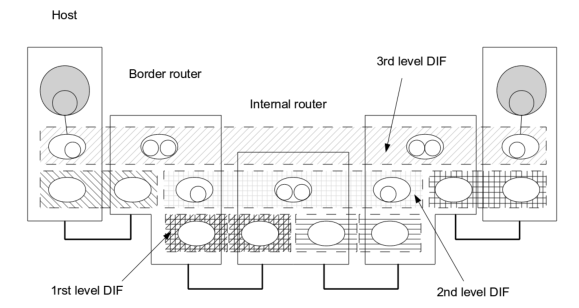
\includegraphics[width=0.6\textwidth]{fig/archs_rina-net.png}
                      \caption{RINA's view of layering.}
                      \label{fig:rina_network}
                    \end{center}
                \end{figure}

                Hence, a DIF is essentially RINA's equivalent of an abstraction layer. However, unlike the traditional network architectures such as the seven-layer ISO/OSI, RINA has only one layer which ``repeats''. This also requires a different kind of notation: instead of using absolute identifier such as \emph{Layer 2} or \emph{Layer 7}, RINA's DIFs are referred to in a relative manner in relation to a specific level, e.g. \emph{(N)-DIF}, \emph{(N+1)-DIF} or \emph{(N-2)-DIF}.

                A computing system may be a member of $<0,n>$ DIFs and has a separate IPC process for each DIF. Each (N)-DIF handles data coming from the (N+1)-DIFs in the same way as from an application.

                A bare minimum for a computer internetwork consists of 3 levels of DIFs and three types of devices: a host, an interior router and a border router. The internetwork is shown in Figure \ref{fig:rina_internetwork}.

                \begin{figure}[H]
                    \begin{center}
                        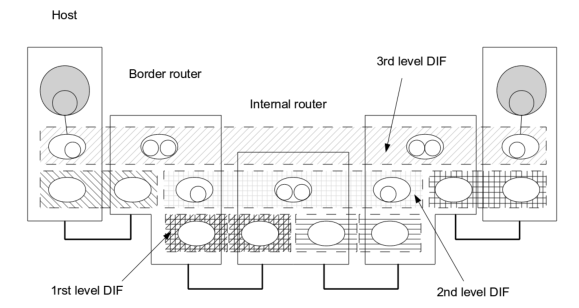
\includegraphics[width=0.6\textwidth]{fig/archs_rina-net.png}
                      \caption{An example of a RINA internetwork with 3 levels of DIFs.}
                      \label{fig:rina_internetwork}
                    \end{center}
                \end{figure}

                As the architecture is recursively scalable, this model could be further expanded: for example, other DIFs could be added on top of the stack in hosts for creating another scope of communication (e.g. for VPN-like facilities).

                Each DIF operates in its own scope isolated from other DIFs of the same level and DIF maintains its own distinct namespace and configuration (such as policies related to security and data transfer). When a computing system wants to communicate with another system inside a foreign DIF, it needs to go through a process of enrollment to the common DIF first.

            \subsubsection{IPC Process}

                Each IPC process executes routing, transport, security/authentication and management functions. The components of an IPC process responsible for providing these functions can be categorized under three decoupled parts operating at separate timescales: \emph{IPC transfer}, \emph{IPC data control} and \emph{IPC management} (see Figure \ref{fig:rina_ipcp}). The behaviour of each part can be configured via policies.

                \begin{figure}[H]
                    \begin{center}
                        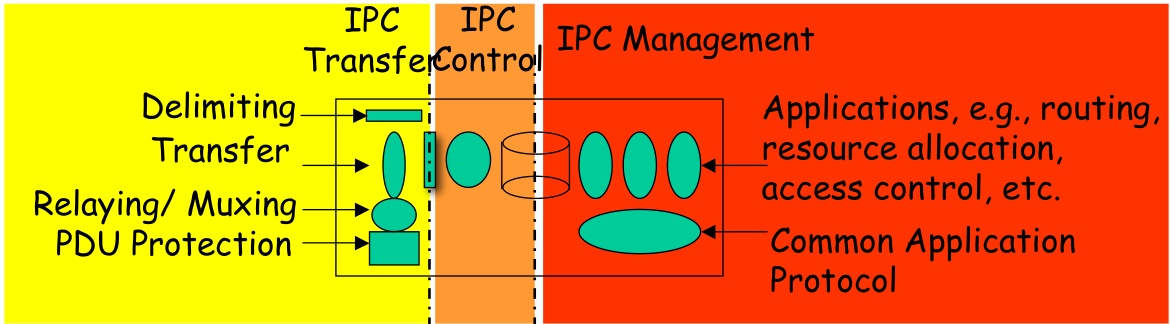
\includegraphics[width=0.6\textwidth]{fig/archs_rina-ipcp.png}
                      \caption{Parts of RINA's IPC process.}
                      \label{fig:rina_ipcp}
                    \end{center}
                \end{figure}

                \begin{itemize}
                    \item IPC transfer consists of following modules:
                    \begin{itemize}
                        \item \textbf{\emph{Delimiting.}} Marks boundaries on incoming (N+1)-SDUs. TODO
                        \item \textbf{\emph{Error and Flow Control Protocol} (EFCP).} A Delta-T \cite{deltat} based protocol that handles individual data flows. EFCPs exchange data via PDUs.
                        \item \textbf{\emph{Relaying and Multiplexing Task} (RMT).} A stateless function that 1) retrieves PDUs from EFCP instances and management tasks and multiplexes then onto a common (N-1)-flow, and 2) takes incoming PDUs and relays them within current IPC or passes them to outgoing port.
                    \end{itemize}
                    \item IPC data control is an optional mechanism handling flow control (for example, TCP-like flow control could be implemented here via appropriate policies). Its functionality is encompassed in the EFCP module.
                    \item IPC management handles management tasks such as routing, resource allocation or access control. It consists of following modules:
                    \begin{itemize}
                        \item \textbf{\emph{Resource Allocator.}} Monitors the resource allocation and performance of the IPC Process and makes adjustments to its operation to keep it within the specified operational range.
                        \item \textbf{\emph{Resource Information Base daemon} (RIB).} The heart of DIF management. Receives/sends management messages and notifies other submodules about management changes.
                    \end{itemize}
                \end{itemize}


            \subsubsection{Addressing}

                Since each DAF operates within its own address scope, the architecture needs to provide means of resolving (N)-application names to addresses of (N-1)-IPC processes. This is achieved via a decentralized distributed \emph{Name Space Manager} (NSM) embedded in each DIF.

                The NSM maintanence is one of the tasks of IPC management; each IPC process keeps track of local registered applications and some of them are specialized to maintain aggregated repository of non-local mapping to serve as forwarders (such processes are called \emph{Repository IPC Processes}).

                \begin{figure}[H]
                    \begin{center}
                        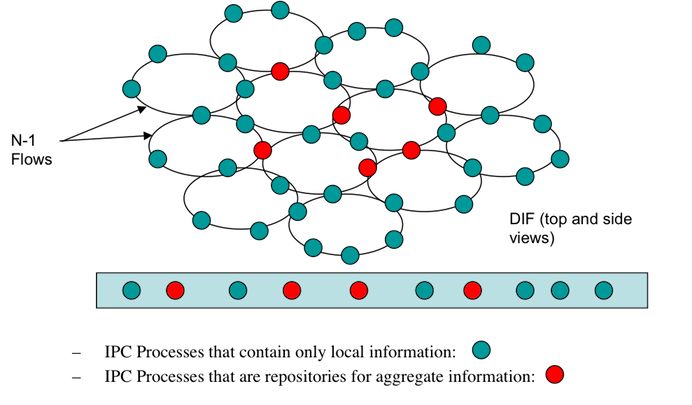
\includegraphics[width=0.6\textwidth]{fig/archs_rina-nsm.png}
                      \caption{Distributed mapping of applications to addresses in a RINA network}
                      \label{fig:rina_nsm}
                    \end{center}
                \end{figure}


            \subsubsection{The Communication Model}\label{archs:rina:communication}

                Every communication in RINA needs to go through the initial process of flow allocation.

                !!! TODO: fix and convert to algorithm2e

                \begin{enumerate}
                    \item App1 requests an IPC connection to App2. This request is handled by ipcProcess1's Flow Allocator.
                    \item The Flow Allocator asks Directory for address of the IPC Process to which App2 is mapped. In this case, it's 2.
                    \item The Flow Allocator asks ipcProcess1's Resource Allocator to find a suitable (N-1)-flow to map the new flow to it. If there isn't any, RA requests an IPC connection to App2.
                    \item The Flow Allocator instructs RIB to send out \texttt{M\_CREATE} request to 2.
                    \item The 2's Flow Allocator instructs RIB to send out \texttt{M\_CREATE\_RESPONSE} request to 1.
                    \item 2's RIB receives the \texttt{M\_CREATE\_RESPONSE}. If it's positive, the Allocate() procedure is ended sucessfully.
                \end{enumerate}

                The applications then exchange data.


            \subsubsection{Policy Separation}

                RINA heavily relies on the design approach of separating mechanism and policy: parts related to authorization of operations and allocation of resources remain constant, while the decisions regarding how to use them are left to policies. In effect, there's only one application protocol (CDAP) and one error and flow control protocol (EFCP). A clear example of the policy separation is EFCP, which is a single mechanism configurable for both reliable and unrealiable data transfer, as opposed to TCP and UDP, which are two distinct mechanisms.

                Thanks to this, RINA can serve as a platform for evaluating multiple approaches to a given problem just by replacing policies. An example can be observed in RINA's approach to routing, which is a policy by itself and provides means for implementing well-known protocols (such as those based on distance vector or link-state algorithms) as well as experimental new paradigms (such as hierarchical and topological routing).

        \subsection{Current State of Implementation}

            ProtoRINA

            IRATI stack

            RINASim, an open-source OMNeT++ implementation of RINA, is being actively developed on FIT BUT.

    \section{Evaluation}

        In the previous sections, we have described 4 new network architectures. This section puts them into context of problems mentioned in chapter \ref{problems} and points out their main strengths and weaknesses.

        \subsection{Named Data Networking}

            The most significant advantage of NDN is its native support for caching all sorts of data inside the network itself. While this should be beneficial mostly for static data such as web pages and images, dynamic content could take advantage of this as well in case of multicasting or packet retransmission on packet loss.

            With its named data paradigm, NDN renders the problems of node naming, mobility and multihoming irrelevant, because data names remain the same no matter the locaton. Same case with security as each data chunk is required to be cryptographically signed by architecture itself.

            The router table size growth presents a challenge as bla bla



\chapter{Forwarding In RINA}\label{forwarding}

    This chapter takes a closer look at components of Recursive InterNetwork Architecture that are related to the implementation target of this thesis. This includes a conceptual description of the forwarding and routing principles in RINA and what role RMT plays in it.

    \section{Distinction of Forwarding And Routing}

        Each IPC process has to solve the forwarding problem: given a set of EFCP PDUs and a number of (N-1)-flows leading to various destinations, to which flow(s) should each PDU be forwarded? In RINA, the decision is handled by the Relaying and Multiplexing task and its forwarding policy. The action may consist of looking up the PDU's destination in a forwarding table (resembling the forwarding mechanism in traditional TCP/IP routers), but it's not a requirement; other experimental forwarding paradigms (such as forwarding based on topological addressing) may not require a forwarding table at all.

        Generating information necessary to do forwarding is one of the tasks of IPC process's Resource Allocator, namely its subcomponent called PDU Forwarding Generator. For this purpose, Resource Allocator generally uses pieces of information provided by other sources, most notably the Routing Policy.

        The Routing Policy exchanges information with other IPC Processes in the DIF in order to generate a next-hop table for each PDU (usually based on the destination address and the id of the QoS class the PDU belongs to). The next-hop table is then converted into a PDU Forwarding Table with input from the Resource Allocator's PDU Forwarding Generator, by selecting an (N-1)-flow for each ``next-hop''. The Routing Policy may resemble distance vector and link-state routing protocols used in today's Internet, but the current research is also aimed at other paradigms such as topological/hierarchical routing, greedy routing or MANET-like routing.


    \section{Relaying and Multiplexing Task}

        \subsection{Formal description}

            Relaying and Multiplexing Task (RMT) has, as its name suggests, two main reponsibilities: relaying and multiplexing of PDUs. The goal of multiplexing is to pass outgoing PDUs (from EFCP instances and management tasks) to the appropriate (N-1)-flows and pass incoming PDUs (from (N-1)-flows) to EFCP instances and management tasks. Relaying handles incoming PDUs from (N-1)-ports\footnote{A handle for an (N-1)-flow, not unlike the traditional BSD socket.} that aren't directed to its IPC process and forwards them to other (N-1)-ports using information provided by its forwarding policy.

            \begin{figure}[H]
                \begin{center}
                    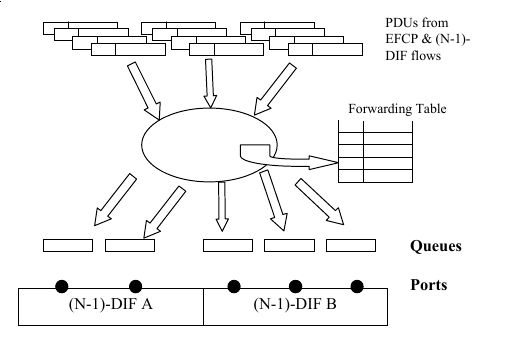
\includegraphics[width=0.6\textwidth]{fig/fwding_rmt-module.png}
                  \caption{Conceptual diagram of Relaying and Multiplexing Task}
                  \label{fig:rmt1}
                \end{center}
            \end{figure}

            RMT instances in hosts and bottom layers of routers usually perform only the multiplexing task, while RMTs in top layers of interior/border routers do both multiplexing and relaying. In addition to that, RMTs in top layers of border routers perform flow aggregation.

            \begin{figure}[H]
                \begin{center}
                    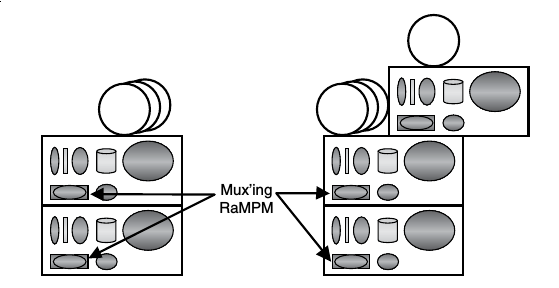
\includegraphics[width=0.6\textwidth]{fig/fwding_rmt-mux.png}
                  \caption{A host with multiplexing RMTs}
                  \label{fig:rmt2}
                \end{center}
            \end{figure}
            \begin{figure}[H]
                \begin{center}
                    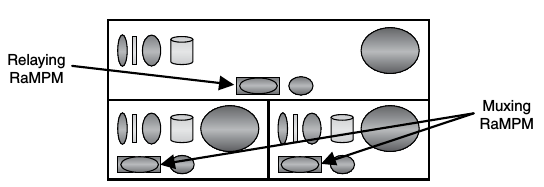
\includegraphics[width=0.6\textwidth]{fig/fwding_rmt-relay.png}
                  \caption{An interior router with two multiplexing RMTs and one relaying RMT}
                  \label{fig:rmt3}
                \end{center}
            \end{figure}
            \begin{figure}[H]
                \begin{center}
                    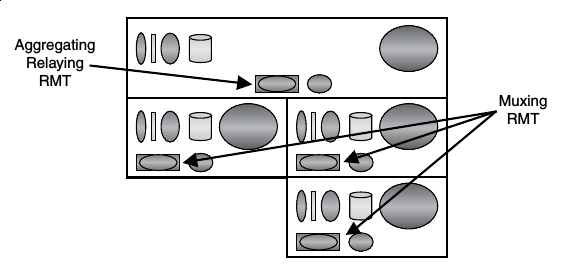
\includegraphics[width=0.6\textwidth]{fig/fwding_rmt-agg.png}
                  \caption{A border router with an aggregating RMT}
                  \label{fig:rmt4}
                \end{center}
            \end{figure}

            Each (N-1)-port handled by RMT has its own set of input and output buffers. The number of buffers, their monitoring, their scheduling discipline and classification of traffic into distinct buffers are all matter of policies.

            RMT is a straightforward high-speed component. As such, most of its management (state configuration, forwarding policy input, buffer allocation, data rate regulation) is handled by the Resource Allocator which makes the decisions based on observed IPC process performance.


        \subsection{Policies}

            Even though Relaying and Multiplexing Task serves as a low-overhead component similar to the traditional view of router data plane, several policies are defined for modifying its behavior.

            \begin{itemize}
                \item RMT scheduling policy. A scheduling algorithm (also commonly known as ``network scheduler algorithm'' or ``queuing discipline'') that determines the order on which input and output buffers are serviced. This policy should be invoked each time a PDU needs to be taken from a queue for processing and works for both input and output directions. Examples of possible algorithms could be FIFO, LIFO or fair queuing.
                \item RMT monitoring policy. A state-keeping queue monitoring algorithm that is invoked each time a PDU enters or leaves a queue. This policy should compute variables to be used in decision process of other policies. Examples of such variables could be average queue length or queue idle time, which are often used by congestion prevention mechanisms.
                \item RMT max queue policy. An algorithm that is invoked each time the number of PDUs waiting in a queue exceeds the queue's threshold. This policy is mostly used for implementing congestion control mechanisms (e.g. by dropping or marking the last PDU in a queue).
                \item Forwarding policy. An algorithm used for deciding where to forward a PDU. The policy is given the PDU's Protocol Control Information (PCI) and in turn returns a set of (N-1)-ports to which the PDU has to be sent. This provides enough granularity to implement multiple communication schemes apart from unicast (such as multicast or load-balancing), because the decision is left to the policy. E.g. a simple forwarding policy would return a single (N-1)-port based on PDU's destination address and QoS-id, whereas in case of a load-spreading policy and multiple (N-1)-ports leading to the same destination, the policy could split traffic by PDUs' flow-ids and always return a single (N-1)-port from the set.
            \end{itemize}



\chapter{Implementation of Relaying and Multiplexing Task}\label{implementation}

    \section{OMNeT++}

        OMNeT++ is an open-source discrete event simulation framework used primarily in the field of network simulation. In this context, the term ``network'' refers to the more general meaning of the word, which means that apart from simulating TCP/IP (especially in conjecture with the INET library) and other computer networks, it also provides means for simulating other networked systems such as on-chip networks or queuing networks. As we're implementing a clean-slate architecture from the ground up, this is an ideal approach.

        OMNeT++ provides a component architecture for models. Components (simple modules) are programmed in C++, then assembled into larger components (compound models) using the high-level language NED. In theory, there are no limits for networks modelled by NED and the only constraint is given by the computing platform processing power.

    \section{RINASim}

        RINASim, developed by networking research group at Faculty of Information Technology of Brno University of technology, is an open-source OMNeT++ library developed for project PRISTINE. The purpose of the library is to provide a framework for building RINA networks and observing their behavior. In the current stage of initial development, RINASim is used primarily by other PRISTINE researchers to experiment with the architecture and efficiently evaluate their working theories.

        The library is open-sourced with MIT licence and publicly hosted by GitHub.

    \section{Process of development}

        Since RINA is still an emerging architecture, speficications for some of its parts (e.g. Resource Allocator) are still being actively worked on and the current implementations aren't yet fit for production purposes. Hence, there wasn't much to rely on when implementing RMT: the specifications were brief, implementation design non-existent and the only existing implementations were providing only a small subset of RMT's functions. Because of this, most of the later phase of development was driven by PRISTINE researchers' feature requests and frequent mutual feedback regarding architectural or implementational issues.

    \section{Implementation Design}

        In RINASim, all functionality of RMT including a policy architecture is encompassed in a single compound module named ``RelayAndMux'' which is present in every IPC process. The module serves for (de)multiplexing, relaying and aggregating PDUs of data flows traversing the IPC processes.

        \begin{figure}[H]
                \begin{center}
                    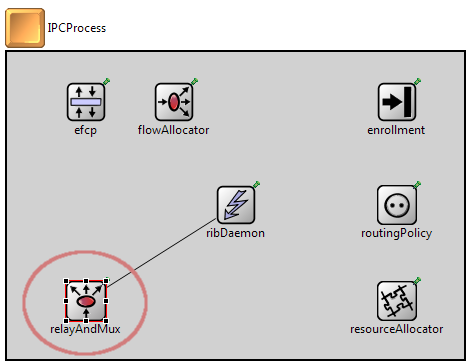
\includegraphics[width=0.7\textwidth]{fig/impl_rinasim-ipcp.png}
                  \caption{RINASim's IPC process}
                  \label{fig:rinasim:ipcp}
                \end{center}
            \end{figure}

        \subsection{Module Structure}

            RelayAndMux consists of multiple simple modules of various types, some of which are instantiated only dynamically at runtime.

            \begin{figure}[H]
                \begin{center}
                    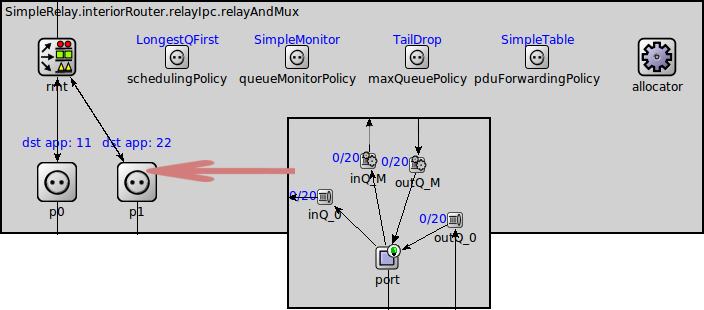
\includegraphics[width=0.6\textwidth]{fig/impl_rinasim-rmt.png}
                  \caption{RelayAndMux module contents}
                  \label{fig:rinasim:rmt}
                \end{center}
            \end{figure}

            \subsubsection{Static modules}
            \begin{itemize}
                \item RMT, the central logic of Relaying And Multiplexing task that decides what should be done with messages passing through the module.
                \item RMTModuleAllocator, a control unit providing an API for adding and deleting instances of dynamic modules (RMTQueue, RMTPort).
                \item SchedulingPolicy, a scheduling policy of an RMT instance.
                \item MonitorPolicy, a monitoring policy of an RMT instance.
                \item MaxQPolicy, a maxqueue policy of an RMT instance.
            \end{itemize}

            \subsubsection{Dynamic modules}
            \begin{itemize}
                \item RMTPort, a representation of one endpoint of an (N-1)-flow.
                \item RMTQueue, a representation of either input or output queue. The number of RMTQueues per RMTPort is determined by Resource Allocator policies.
                \item RMTPortWrapper, a compound module encapsulating an (N-1)-port and its queues.
            \end{itemize}

            \begin{figure}[H]
                \begin{center}
                  \makebox[\textwidth]{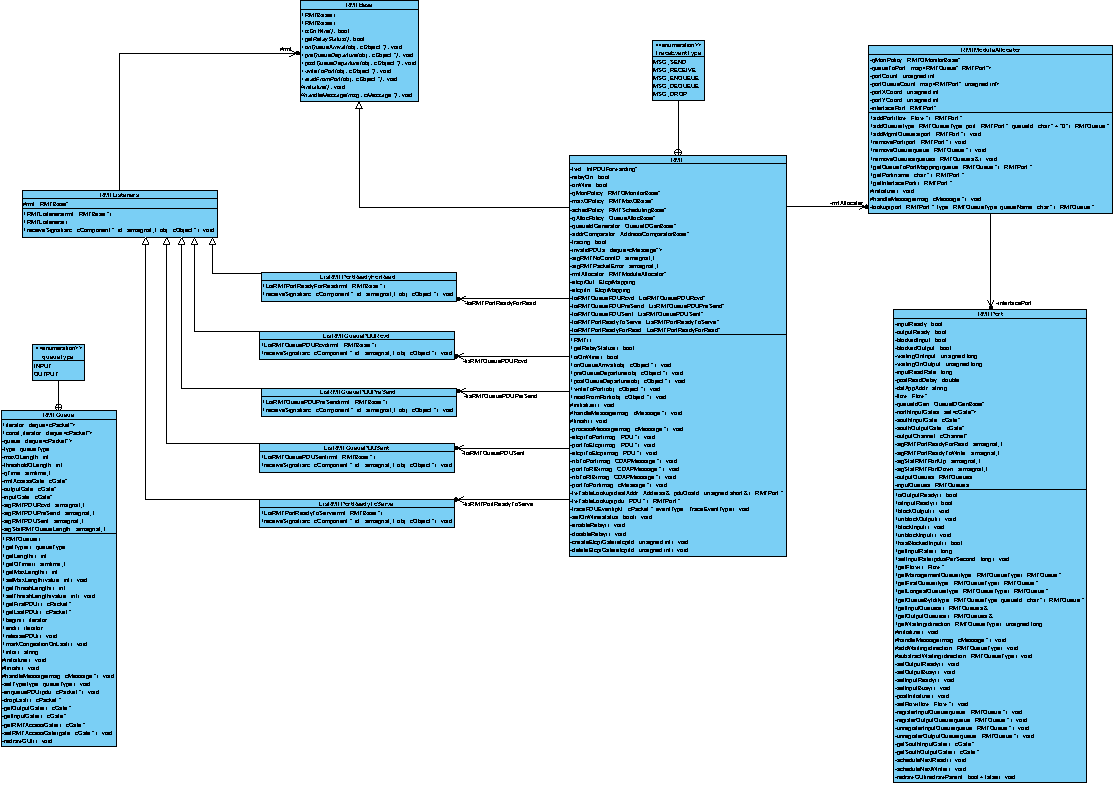
\includegraphics[width=\textwidth]{fig/impl_rmt-erd.pdf}}
                  \caption{RMT class diagram}
                  \label{fig:rmt-erd}
                \end{center}
            \end{figure}

        \subsection{Module Parameters}
            The RMT module contains several user-configurable parameters that can be used to alter its behavior. These are presented in Table \ref{fig:rmt_params}.

            \begin{table}[H]
                \begin{center}
                  \begin{tabular}{ | r | r | l | }
                    \hline
                    data type & name & function \\
                    \hline
                    \texttt{string} & \texttt{schedPolicyName} & name of the desired scheduling policy \\
                    \texttt{string} & \texttt{qMonitorPolicyName} & name of the desired monitoring policy \\
                    \texttt{string} & \texttt{maxQPolicyName} & name of the desired max queue policy \\
                    \texttt{string} & \texttt{ForwardingPolicyName} & name of the desired forwarding policy \\
                    \texttt{int} & \texttt{defaultMaxQLength} & default maximum length of instantiated queues \\
                    \texttt{int} & \texttt{defaultThreshQLength} & default threshold length of instantiated queues \\
                    \texttt{bool} & \texttt{pduTracing} & a switch for turning on PDU tracefile generation \\
                    \hline
                  \end{tabular}
                  \caption{RMT module parameters.}
                  \label{fig:rmt_params}
                \end{center}
            \end{table}

        \subsection{Module Workflow}

            The core function of RMT is driven by two algorithms: the decision algorithm and the scheduling algorithm.

            The decision algorithm decides what to do with the incoming PDU and executes appropriate policies. A state diagram representation can be seen in Figure \ref{fig:rmt-fsm}. It's implemented by \texttt{handleMessage()} and methods that are subsequently called from it (\texttt{portToEFCPI()}, \texttt{portToPort()} etc.).

            \begin{figure}[H]
                \begin{center}
                  \makebox[\textwidth]{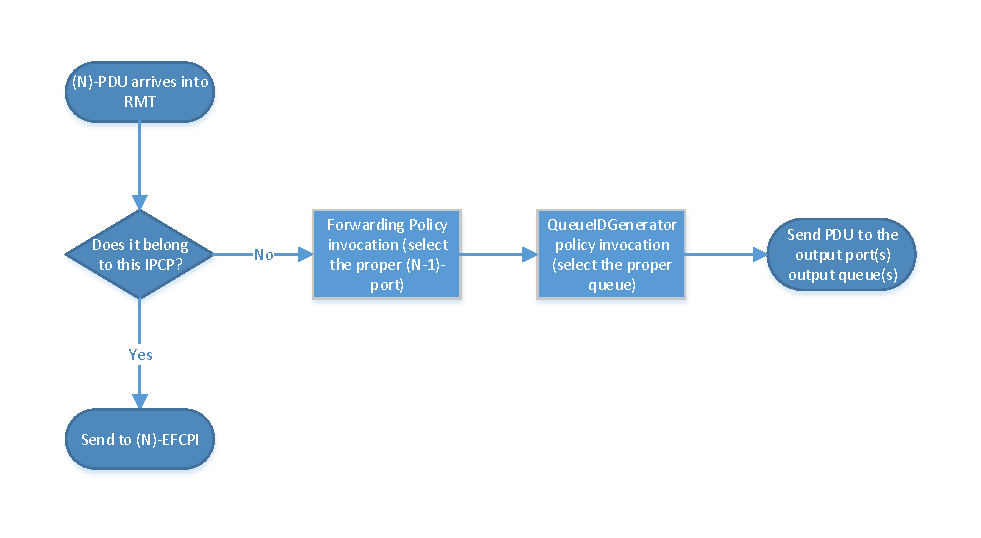
\includegraphics[width=\paperwidth/3]{fig/impl_rmt-decision.pdf}}
                  \caption{The core RMT decision process}
                  \label{fig:rmt-fsm}
                \end{center}
            \end{figure}

            The scheduling algorithm ensures continuous invocation of the scheduling policy whenever there are PDUs waiting in queues. A petri net representation can be seen in Figure \ref{fig:sched-petri}. The decision of what queue should be processed next is left to the policy. The algorithm is implemented by methods \texttt{onQueueArrival()}, \texttt{postQueueDeparture()}, \texttt{writeToPort()} and \texttt{readToPort()}.

            \begin{figure}[H]
                \begin{center}
                  \makebox[\textwidth]{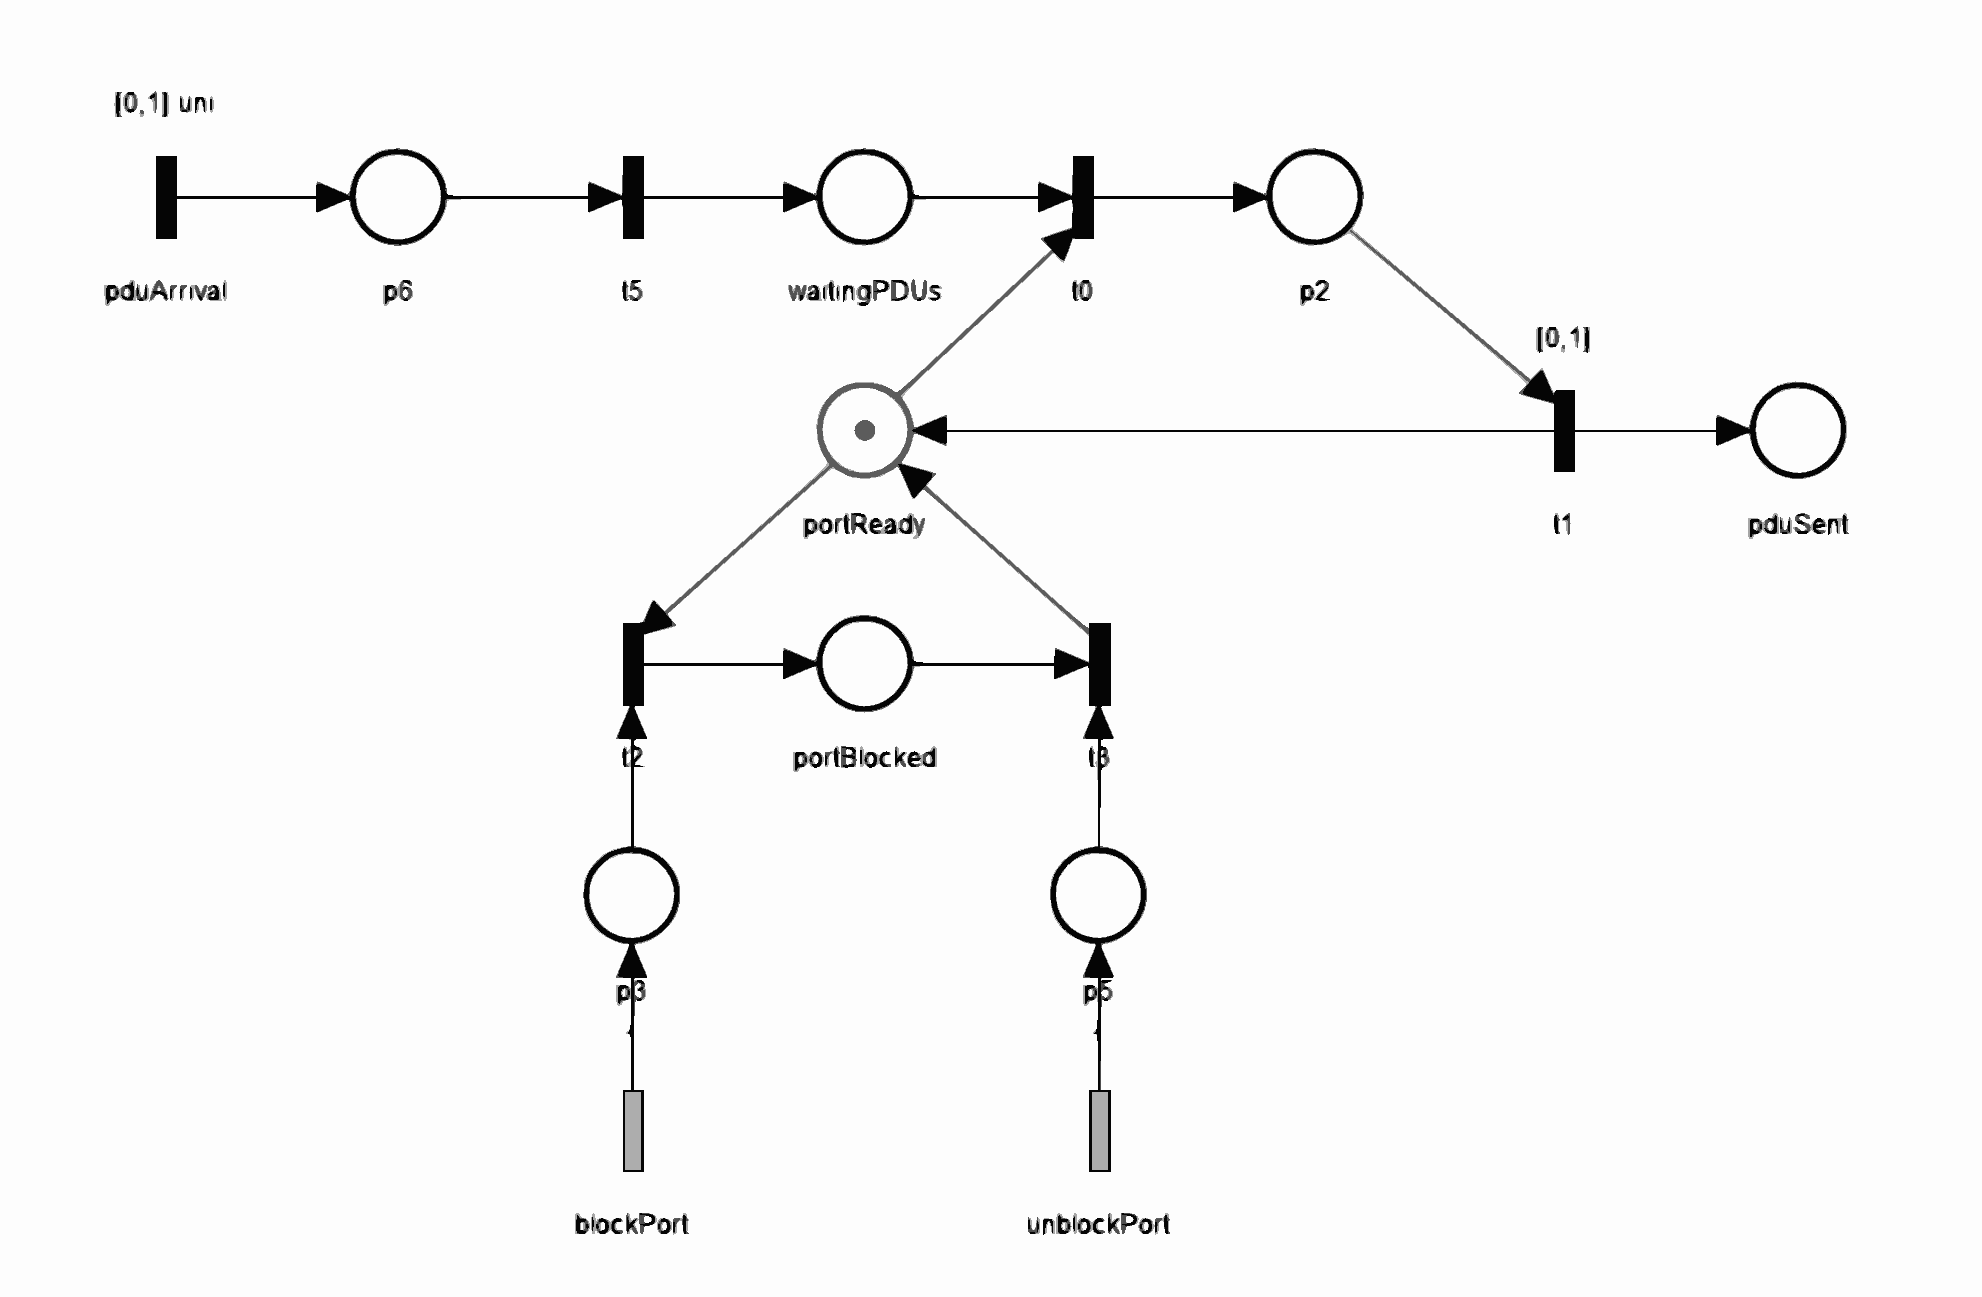
\includegraphics[width=\paperwidth/2]{fig/impl_rmt-sched.pdf}}
                  \caption{The RMT scheduling procedure}
                  \label{fig:sched-petri}
                \end{center}
            \end{figure}

        \subsection{Module Management}\label{implementation:mgmt}

            RMT's purpose in an IPC process is fairly straightforward: providing a stateless function for relaying PDUs to their predetermined destinations and multiplexing PDUs of multiple data flows onto a common predetermined medium. The entire management of the RMT is decoupled and exercised by the Resource Allocator.

            As Resource Allocator lacked any more concrete specifications at the time of implementation, I have designed a set of management functions, some of which are customizable by policies.

            \subsubsection{Initial RMT Mode Setup}

                When a RMT instance is located inside a bottommost IPC process that doesn't work with any further (N-1)-IPC processes, the RMT is switched to an \texttt{onWire} mode that functions over a single serializing medium instead of an IPC connection.

                If a RMT is located inside an IPC process that has the \texttt{relay} configuration parameter configured as \texttt{true}, the RMT's Relaying Task is enabled by calling \texttt{enableRelay()}. The default value of the \texttt{relay} parameter is \texttt{true} in top layers of routers, \texttt{false} everywhere else.

            \subsubsection{Forwarding Table Management}

                The content of the PDU forwarding table is generated by the PDU Forwarding Generator policy module which generally accepts input from other sources such as the Routing policy module.

            \subsubsection{Queue allocation}

                PDUs traversing an (N-1)-port may be momentarily buffered in input or output queues; the number of input and output queues per (N-1)-port and assignment of traffic classes to queues (e.g. all-in-one or fair queuing)
                is determined by two Resource Allocator policies.

                \begin{itemize}
                    \item QueueAlloc: The (N-1)-port queue allocation strategy. The interface contains a set of event hook methods (\texttt{onPolicyInit}, \texttt{onNM1PortInit}, \texttt{onNFlowAlloc}, \texttt{onNFlowDealloc}) that allow the user to specify how many queues should be allocated or deallocated in response to which events.
                    \item QueueIDGen: A companion classification policy to QueueAlloc which generates a queue ID for given PDU. This policy is used by RMT when it needs to determine which of the port's queue should a PDU be placed in.
                \end{itemize}

            \subsubsection{(N-1)-port creation \& removal}

                Since Resource Allocator manages (N-1)-flows leading to other IPC processes, it also provides (N-1)-ports (or handles) for RMT.

            \subsubsection{(N-1)-port data rate control}

                In some scenarios, it may be required for an (N-1)-port to cease/slow down sending or providing more data because of congestion. Resource Allocator can momentarily disable or slow down data rate on distinct ports if this is required by EFCP instances.


        \subsection{Statistics Collection}

            OMNeT++ modules provide means for declaring scalar or vector NED variables used for statistics collection. Processing of such statistical data (e.g. generating summaries and graphs) is decoupled from the act of data collection itself, so it's up to the user to pick out which data he wants to work with.

            Since the Relaying and Multiplexing Task is the shared point of data flow traversal in the IPC process, it's well-suited for monitoring data flow performance. Several statistical variables have been defined for this very purpose:

            \begin{itemize}
                \item (N-1)-port PDU traversal count. Two scalar variables for both input and output containing the number of PDUs transferred through the port in each direction.
                \item RMT queue length. A vector variable documenting number of PDUs in a queue over time.
                \item RMT queue drop count. A scalar variable providing the number of PDUs dropped by a queue.
            \end{itemize}

            Multiple examples of graphs generated from the variables can be seen in chapter \ref{testing}.

    \section{Sample policy implementations}

        As Relaying And Multiplexing follows the design principle of separation of mechanism and policy, most of its complexity lies in the policies. Hence, to demonstrate the use of RMT's policy framework, I have implemented a diverse set of simple RMT policies.

        \begin{itemize}
            \item \textbf{Scheduling policy}
            \begin{itemize}
                \item LongestQFirst: pick the queue which contains the most PDUs.
            \end{itemize}
            \item \textbf{Monitoring policy}
            \begin{itemize}
                \item REDMonitor: used in conjecture with REDDropper; Random Early Detection implementation.
            \end{itemize}
            \item \textbf{Max queue policy}
            \begin{itemize}
                \item ECNMarker: If queue size $\geq$ threshold, apply ECN marking on new PDUs; if size $\geq$ max, drop.
                \item ReadRateReducer: If queue size $\geq$ allowed maximum, stop receiving data from input ports.
                \item REDDropper: Used in conjecture with REDMonitor; Random Early Detection implementation.
                \item TailDrop: If queue size $\geq$ allowed maximum, drop new PDUs.
                \item UpstreamNotifier: If queue size $\geq$ allowed maximum, send a notification to the PDU sender.
            \end{itemize}
            \item \textbf{PDU Forwarding policy}
            \begin{itemize}
                \item SimpleTable: A table with \{(dstAddr, QoS) $\rightarrow$ port\} mappings.
            \end{itemize}
        \end{itemize}

        To demonstrate the abilities of Resource Allocator's RMT management, I have also implemented an additional set of management policies (introduced in section \ref{implementation:mgmt}).

        \begin{itemize}
            \item \textbf{QueueAlloc}
            \begin{itemize}
                \item QueuePerNFlow: Maintain a queue for each (N)-flow.
                \item QueuePerNQoS: Maintain a queue for each (N)-QoS cube.
            \end{itemize}
            \item \textbf{QueueIDGen}
            \begin{itemize}
                \item IDPerNFlow: Companion policy for QueueAlloc::QueuePerNFlow.
                \item IDPerNQoS: Companion policy for QueueAlloc::QueuePerNQoS.
            \end{itemize}
        \end{itemize}


\chapter{Testing and Evaluation}\label{testing}

    I have created a set of basic network topologies to demonstrate the implementation's features. The following tests put them into use.
    Each test case contains a description of RMT-related events that happen during simulation. Each type of event is described only once to prevent needless repetition.

    For purposes of testing, RINASim contains a ping-like application called \texttt{AEPing} that can serve as both sender and receiver of a ping-like data frame. Each of the following scenarios consists of a NED topology and two instances of AEPing on different hosts. The first instance with application name \texttt{App1} allocates a flow to the other instance with application name \texttt{App2}, pings the other instance multiple times in sucession and then deallocates the flow. The simulation times of flow allocation, ping send events and flow deallocation are configurable via the AEPing NED module.

    Additionally, each channel connecting two hosts is configurable to simulate postponed message delivery based on its bandwidth or fixed delay. To keep the format of timestamps simple, channels in the following examples operate with a fixed delay in seconds.

    \section{Basic multiplexing}

        This example presents the multiplexing function of RMT in a simple scenario.

        \subsection{Topology}

            The TwoCS topology is the most basic example of a computer network. It consists of two interconnected hosts, each with a single application and two IPC processes. More on Figure \ref{fig:examples:muxing:events:topology}.

            \begin{figure}[H]
                \begin{center}
                    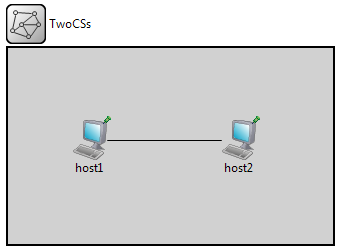
\includegraphics[width=0.6\textwidth]{fig/examples-twocs.png}
                  \caption{TwoCS simulation scenario}
                  \label{fig:examples:muxing:events:topology}
                \end{center}
            \end{figure}

        \subsection{Scenario}

            The configuration of this simulation scenario is described in Table \ref{fig:examples:muxing:events}.

            \begin{table}[H]
                \begin{center}
                  \begin{tabular}{ | r | l | l | }
                    \hline
                    module & configuration directive & value \\
                    \hline
                    \texttt{host1}'s \texttt{AEPing} & flow allocation & 10 s \\
                    \texttt{host1}'s \texttt{AEPing} & first ping & 35 s \\
                    \texttt{host1}'s \texttt{AEPing} & flow deallocation & 200 s \\
                    \texttt{host1}'s \texttt{AEPing} & number of pings & 10 \\
                    \texttt{host1}$\rightarrow$\texttt{host2} channel & delay & 2 s \\
                    \hline
                  \end{tabular}
                  \caption{Configuration of the scenario.}
                  \label{fig:examples:muxing:events}
                \end{center}
            \end{table}

        \subsection{Simulation}

            What follows is a simplified description of events related to RMT instances.

            \begin{itemize}
            \item \textbf{t=0}: The RMT instances undergo their initial setup. For the bottom IPC processes in both hosts, this consists of creating a RMTPort instance named \texttt{PHY} and its queues. Since the QueueAlloc policy is set to \texttt{SingleQueue}, the following queues are created: \texttt{outQ\_M} (management output), \texttt{inQ\_M} (management input), \texttt{outQ\_0} (data output) and \texttt{inQ\_0} (management input).

            \item \textbf{t=10}: \texttt{App1} invokes \emph{Allocate(\texttt{App2})}. This in turn causes \texttt{IPC11}'s Resource Allocator to invoke \emph{Allocate(\texttt{IPC2})}.

                The RIB in \texttt{IPC11} sends out an \texttt{M\_CREATE} request addressed to \texttt{IPC22}. RMT stores the PDU to the \texttt{PHY}'s queue \texttt{outQ\_M}.

                The arrival of PDU into the queue causes invocation of the active monitoring policy and MaxQ policy. If the MaxQ policy hasn't caused the PDU to be dropped, the scheduling policy is invoked.

                The scheduling policy decides to release the PDU from \texttt{outQ\_M}. The PDU traverses through the port and gets sent to the other host via the medium.

            \item \textbf{t=12}: \texttt{IPC2}'s RMT receives the PDU on port \texttt{PHY}. As this is a management PDU, it's stored into the management input queue \texttt{inQ\_M}.

                The arrival of PDU into the queue causes invocation of the active monitoring policy and MaxQ policy. If the MaxQ policy hasn't caused the PDU to be dropped, the scheduling policy is invoked.

                The scheduling policy decides to release the PDU from \texttt{inQ\_M}. The PDU travels into the dispatcher which relays the PDU to the RIB daemon.

                The RIB daemon sends out an \texttt{M\_CREATE\_RESPONSE} frame to \texttt{IPC1}.

            \item \textbf{t=14}: The \texttt{IPC1}'s RIB daemon receives the \texttt{M\_CREATE\_RESPONSE} request and the \emph{Allocate(\texttt{IPC2})} procedure is sucesfully completed. The new connection is mapped to a newly instantiated RMTPort called \texttt{p0} and the previously suspended \emph{Allocate(\texttt{App2})} procedure is triggered to continue and carry out the same series of events, only one level higher and using \texttt{IPC1}1's port \texttt{p0} and its data queues.

            \item \textbf{t=18}: The \emph{Allocate(\texttt{IPC2})} procedure is sucessfully completed and \texttt{App1} is now connected to \texttt{App2}.

            \item \textbf{t=35}: In \texttt{host1}, \texttt{App1} sends out the first ping. The ping traverses RMTs in \texttt{IPC11} and \texttt{IPC1} and then it's sent to the medium. This is repeated nine times in the following 9 seconds.

            \item \textbf{t=37}: In host2, \texttt{IPC0}'s port \texttt{PHY} receives the first ping. The ping traverses RMTs in \texttt{IPC2} and \texttt{IPC22} and then it's handed to App2. This is repeated nine times in the following 9 seconds.

            \item \textbf{t=200}: App1 invokes \emph{Deallocate(\texttt{App2})}.

            \item \textbf{t=202}: The connection between \texttt{App1} and \texttt{App2} is deallocated.
            \end{itemize}

        \subsection{Evaluation}

            The implementation reflects the expected behavior.

    \section{Basic Relaying}

        This example presents the relaying function of RMT in a simple scenario.

        \subsection{Topology}

            The SimpleRelay topology is the most basic example of a computer network with a relaying device. It consists of two hosts interconnected by a router with three IPC processes. More on Figure \ref{fig:examples:simplerelay}.

            \begin{figure}[H]
                \begin{center}
                    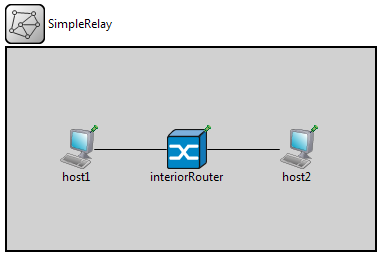
\includegraphics[width=0.6\textwidth]{fig/examples-simplerelay.png}
                  \caption{SimpleRelay network topology.}
                  \label{fig:examples:simplerelay}
                \end{center}
            \end{figure}

        \subsection{Scenario}

            The simulation scenario is described in table

            \begin{figure}[H]
                \begin{center}
                  \begin{tabular}{ r | l }
                    time & event \\
                    \hline
                    10s & App1 begins allocation of an IPC connection to App2. \\
                    35s & App1 begins sending 10 pings (one per second) to App2. \\
                    200s & App1 begins deallocation of IPC connection with App2. \\
                    \hline
                  \end{tabular}
                  \caption{RMT module parameters.}
                  \label{fig:examples:relaying}
                \end{center}
            \end{figure}

        \subsection{Simulation}

        \subsection{Evaluation}

    \section{Basic Congestion Control}

        This scenario presents an example of porting a legacy congestion control algorithm into RINA by converting it into RMT policies. The algorithm in question is Random Early Detection (RED) which is implemented as a set of a monitoring policy and a maxQ policy. Additionaly, this scenario presents the port blocking subsystem.

        \begin{figure}[H]
            \begin{center}
                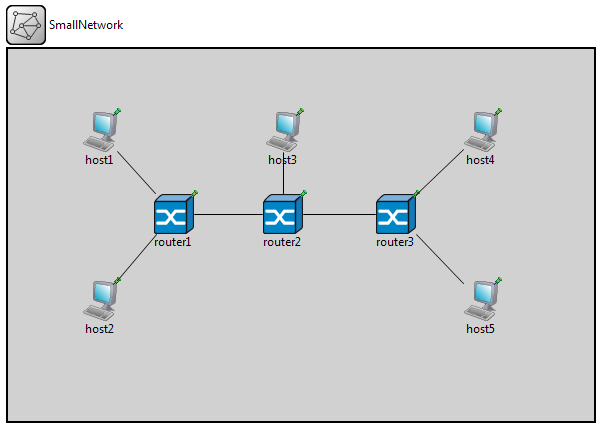
\includegraphics[width=0.6\textwidth]{fig/examples-smallnetwork.png}
              \caption{SmallNetwork simulation scenario}
              \label{fig:examples:red}
            \end{center}
        \end{figure}

        \subsection{Topology}

        \subsection{Simulation}

        \subsection{Evaluation}


\chapter{Conclusion}\label{conclusion}

    In this thesis, I have delved into the field of network architecture research.

    The goal of this thesis was to contribute to prototyping attempts of one of the presented network architectures, RINA. This task has been sucessfully completed by implementing RINA's Relaying and Multiplexing Task into an existing library for simulation tool OMNeT++.

    To be able to describe the principles of new network architectures and analyze their contributions, I needed to gain understanding of the driving factors behind their inception. This has been achieved by studying the Internet and its history to learn about choices that lead to its current state, as well as its problems. I have noticed that some of the drawbacks of its architectural design have been recognized right at the beginning of its inception.

    To understand RINA, I had to adapt to its paradigm shift which abandons most of today's widely recognized principles of computer networking.

    The implementation part of this thesis required me to learn about OMNeT++ programming framework and the RINASim library.

    The resulting solution is currently in use by multiple research groups for modelling RINA networks and experimenting with various policies.

    \section{Future Development}

    The resulting implementation provides users with a policy framework that allows them to experiment with virtually unlimited number of approaches to forwarding and congestion control in RINA. Therefore, future development lies mainly in expansion of the policy set. Several examples of such new policies written by RINA researchers are already available in the source code repository at the time of writing this thesis. Such examples usually explore new directions in the areas of congestion control, routing and distributed resource allocation.

